\section{Framework}

\subsection{Architettura Generale}
L'architettura che abbiamo scelto per la progettazione del framework è del tipo Model-View-Controller (MVC). La parte della View consiste nell'interfaccia grafica per l'utente (GUI) che permetterà la gestione di elementi grafici. La parte di Model permetterà la gestione degli elementi funzionali ed è composta dalla bubble memory e dalle API. La parte di Controller che consiste nella bubble generica si occuperà di gestire l'aggiornamento della GUI e l'invio degli input dell'utente agli elementi funzionali.

\begin{figure}[H]
	\centering
	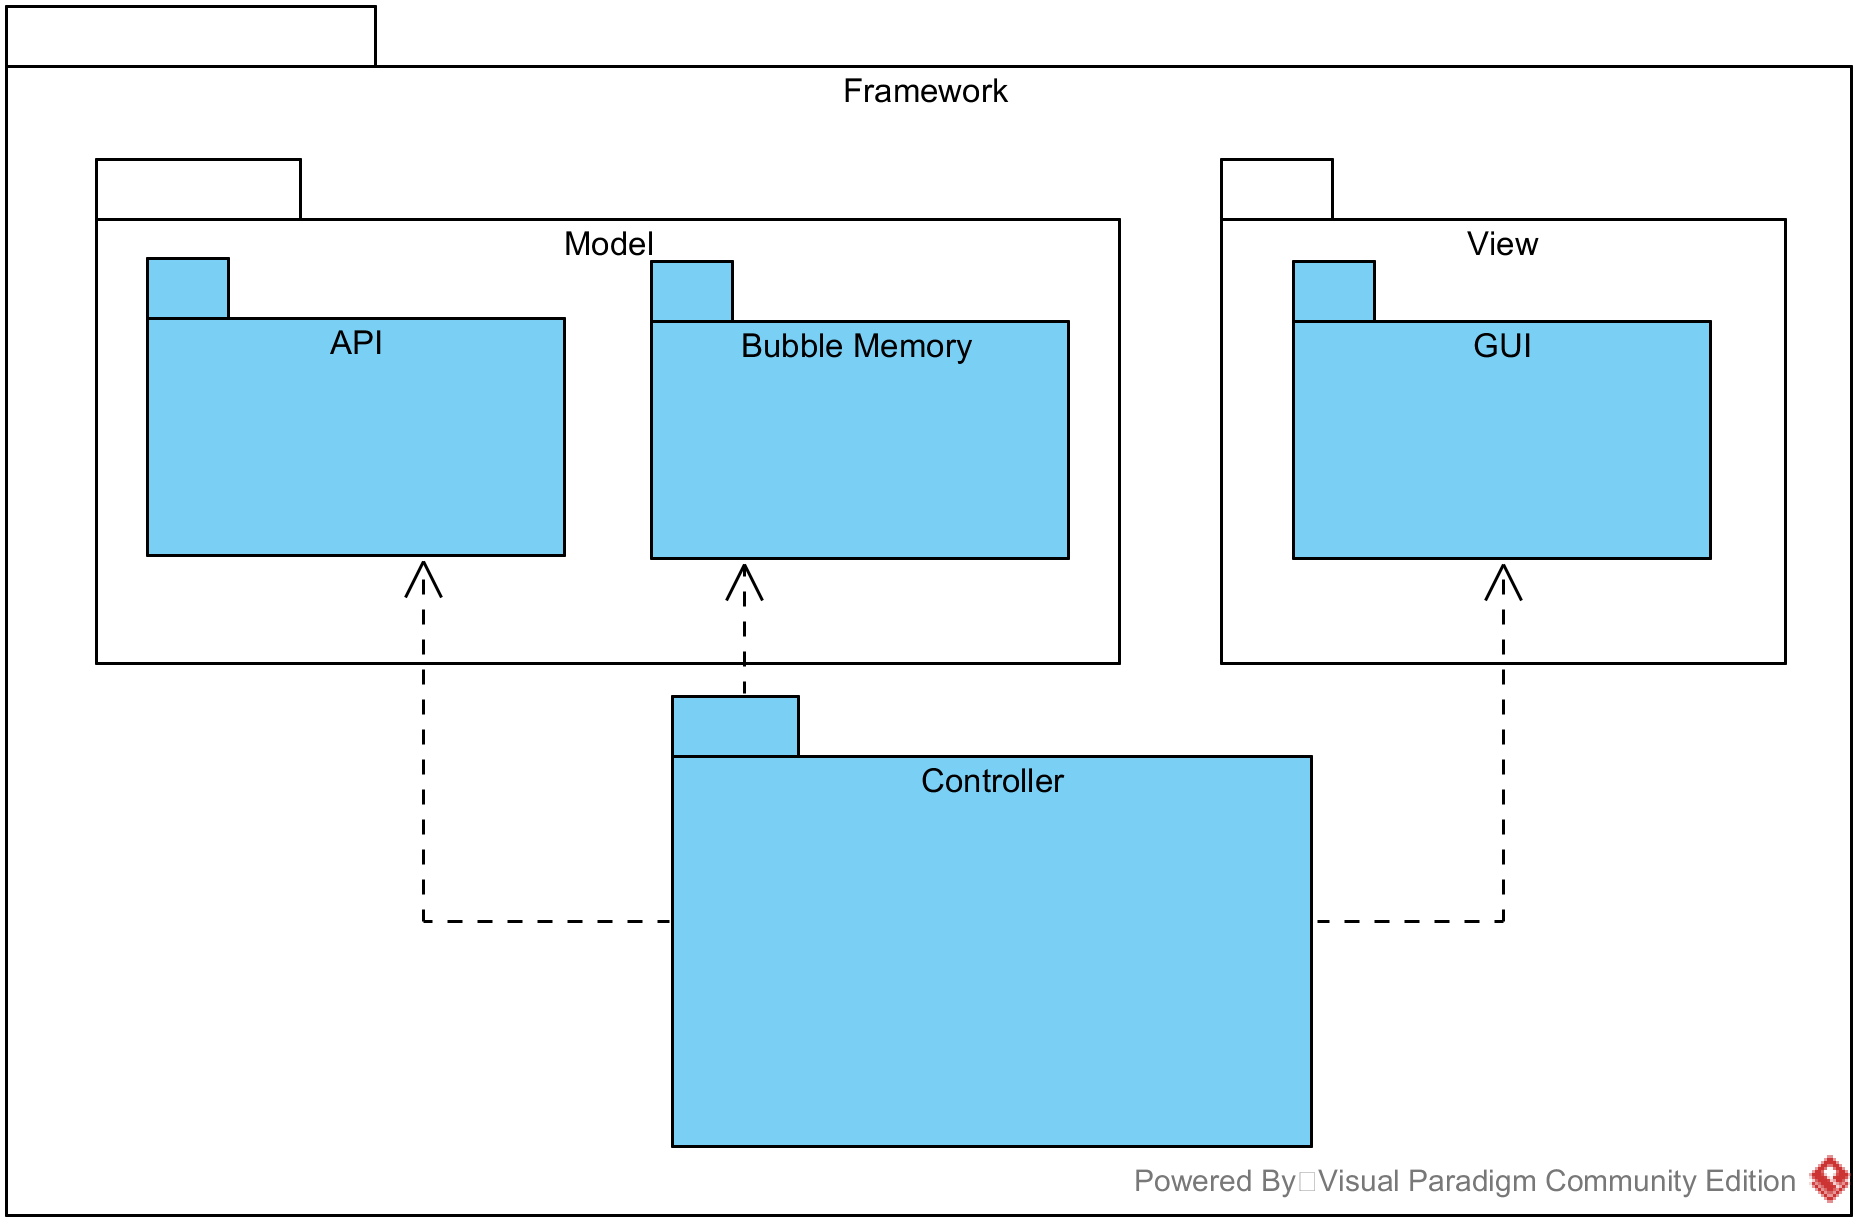
\includegraphics[width=14cm]{diagrammi_img/classi_e_package/framework.png}
	\caption{Architettura framework}
\end{figure}

\subsection{Model}
Nella scomposizione logica in MVC la parte relativa al model, ossia la business logic dell'applicativo, è delegata alla bubble memory e ai pacchetti di metodi che compongono il framework. Questi metodi possono essere combinati tra loro e legati all'interfaccia grafica mediante il controller.

\begin{figure}[H]
	\centering
	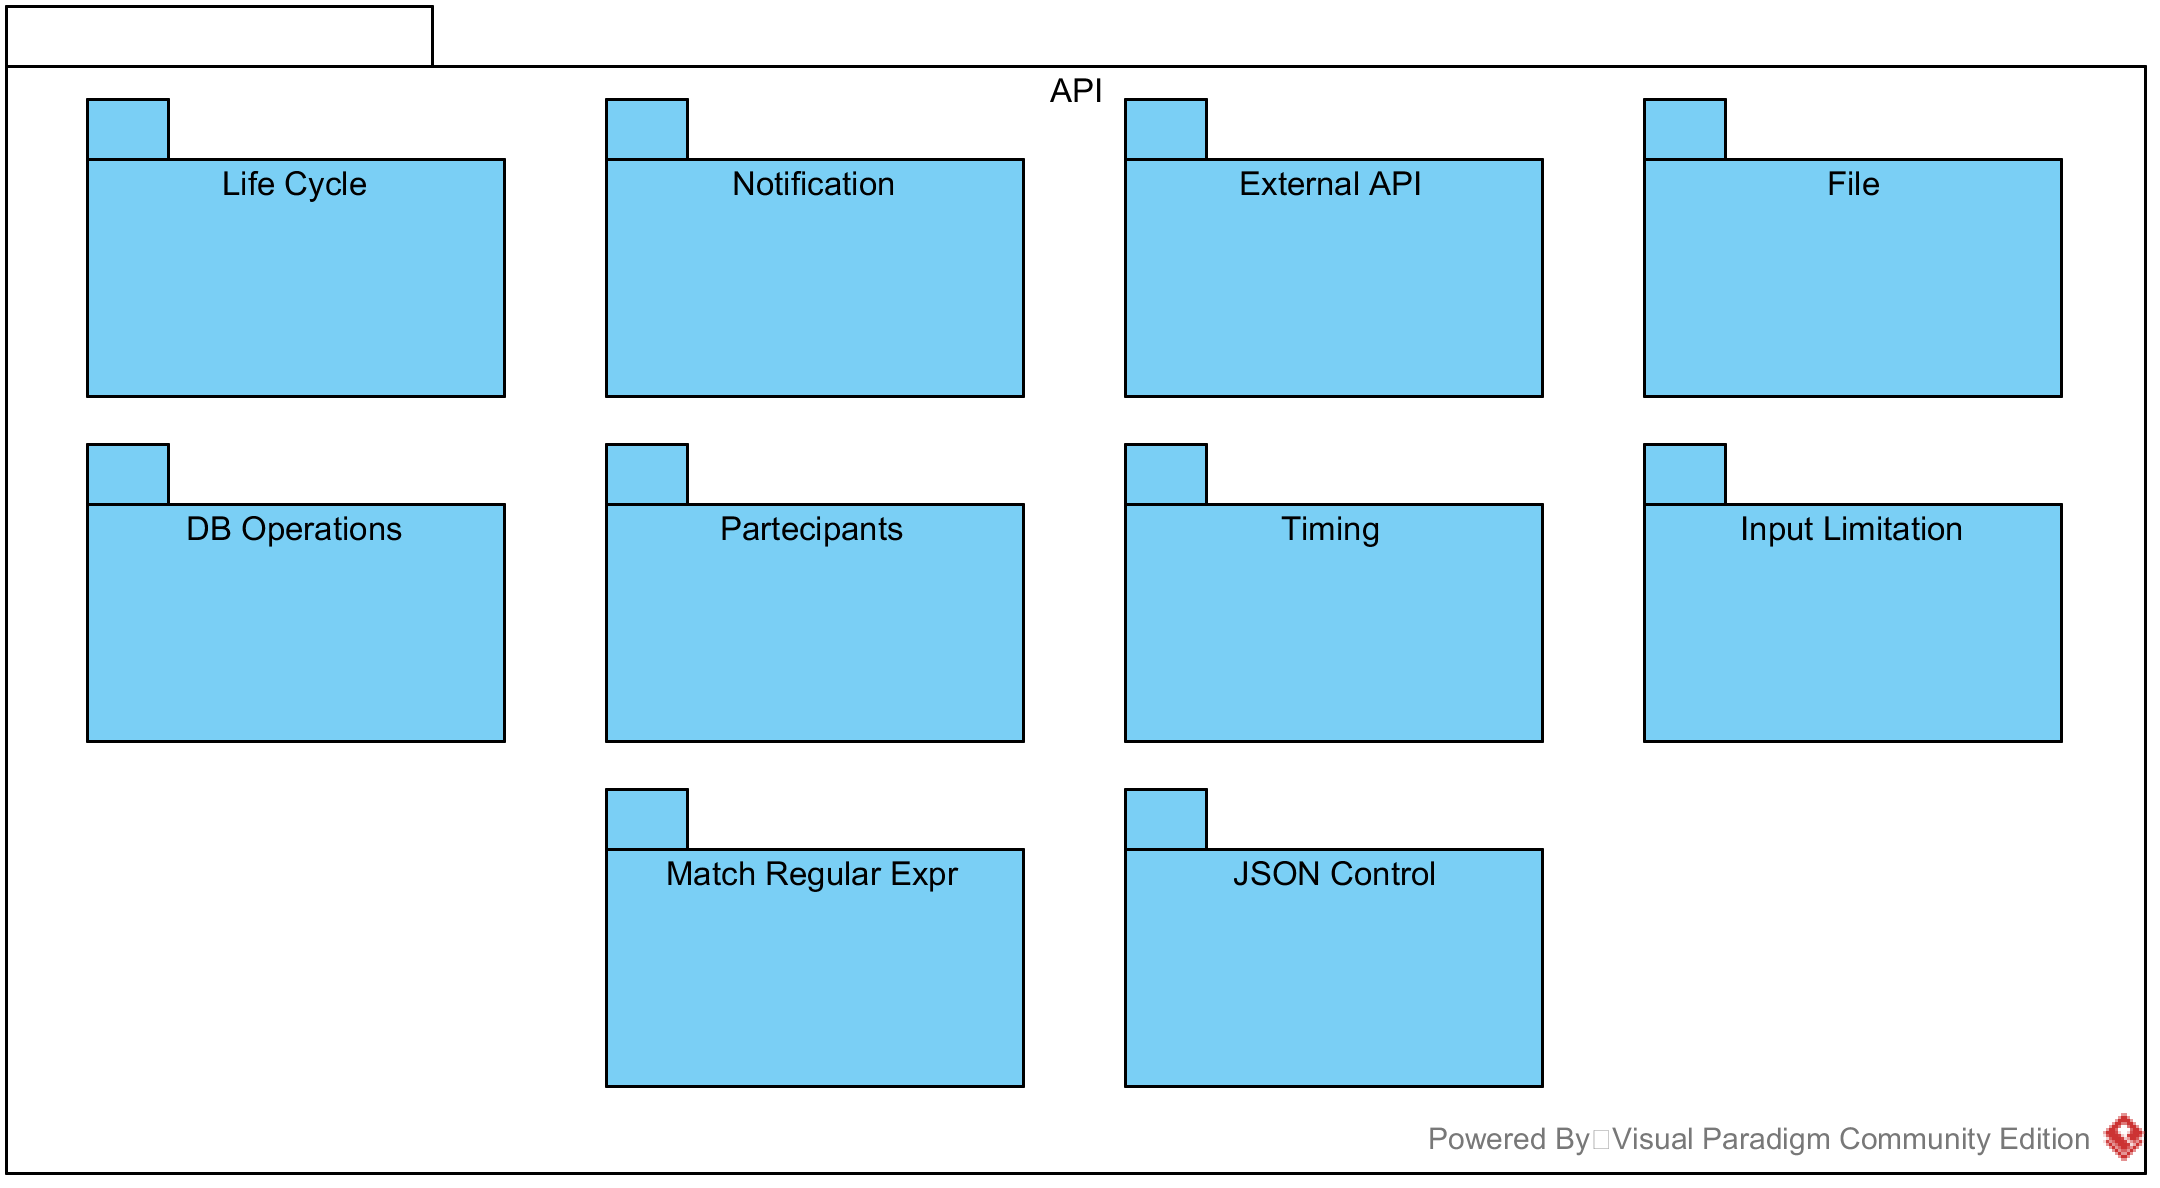
\includegraphics[width=14cm]{diagrammi_img/classi_e_package/framework_api_package.png}
	\caption{Architettura framework model api}
\end{figure}

\subsection{Bubble Memory}
La componente di bubble memory gestisce la parte di persistenza della bubble in locale, tenendo traccia di variabili e del loro valore, incluso lo stato della bubble. La bubble memory è strutturata come un oggetto JavaScript, non avendo così vincoli relativamente al tipo di informazioni che è possibile inserire al suo interno.

\begin{samepage}
\subsubsection{BubbleMemory}\label{fm-memory}
\nopagebreak
\begin{figure}[H]
	\centering
	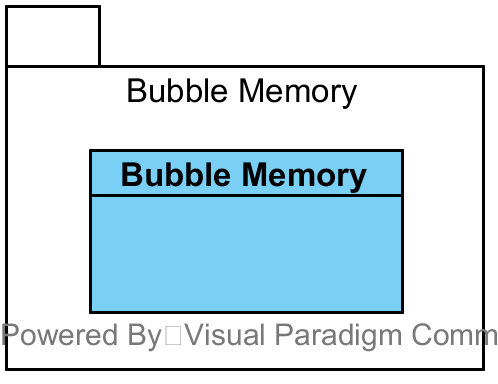
\includegraphics[height=5cm]{diagrammi_img/classi_e_package/bubble_memory.png}
	\caption{BubbleMemory}
\end{figure}	
\end{samepage}
\textbf{Descrizione:}\\
La bubble memory è la parte che si occupa di immagazzinare i dati relativi alla bubble. \\
\textbf{Scopo:}\\
Verrà usato come contenitore per le variabili degli elementi di input e output e lo stato della bubble.

\subsection{API del framework}
Ciascun package contiene classi di metodi, i quali garantiscono funzionalità che possono essere combinate nel corpo della bubble al fine di determinarne la business logic.\\
Data la natura del progetto non sono rappresentate connessioni tra i vari package riportati nel diagramma sopra, in quanto, essendo questa parte del prodotto un framework volto a garantire la possibilità di creare bubble interattive a sviluppatori terzi, verrà perseguito l'obiettivo di massimizzare l'indipendenza tra queste funzionalità in maniera tale da altrettanto massimizzare le possibilità di riutilizzo delle stesse.

\subsubsection{Package interni}

\begin{samepage}
\paragraph{Api\-::Life\-Cycle}\label{api-ciclovita}\mbox{}\\
\nopagebreak
\begin{figure}[H]
	\centering
	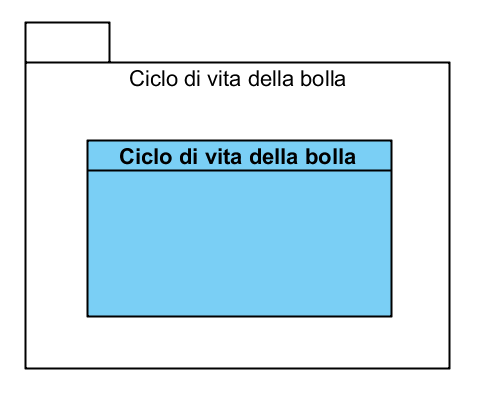
\includegraphics[height=5cm]{diagrammi_img/classi_e_package/api_vitabolla.png}
	\caption{Api\-::Life\-Cycle}
\end{figure}
\end{samepage}
\textbf{Descrizione:}\\ 
Lo scopo di questo package è di gestire le operazioni legate al ciclo di vita della bubble.\\
\textbf{Utilizzo:}\\
Si occupa di controllare la durata di vita della bubble interrompendo il funzionamento dopo un tempo prefissato.\\

\begin{samepage}
\paragraph{Api\-::Notification}\label{api-notifica}\mbox{}\\
\nopagebreak
\begin{figure}[H]
	\centering
	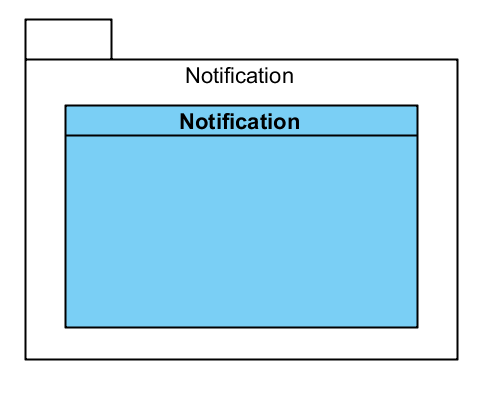
\includegraphics[height=5cm]{diagrammi_img/classi_e_package/api_notifica.png}
	\caption{Api\-::Notification}
\end{figure}
\end{samepage}
\textbf{Descrizione:}\\ 
I metodi presenti all'interno del package di notifica hanno lo scopo di creare e mostrare agli utenti delle notifiche collegate con le azioni della bubble. Se incluso nella bubble sarà possibile notificare del testo in modo statico.\\
\textbf{Scopo:}\\
Si occupa della gestione di notifiche statiche all'utente.\\

\begin{samepage}
\paragraph{Api\-::External\-Api}\label{api-esterne}\mbox{}\\
\nopagebreak
\begin{figure}[H]
	\centering
	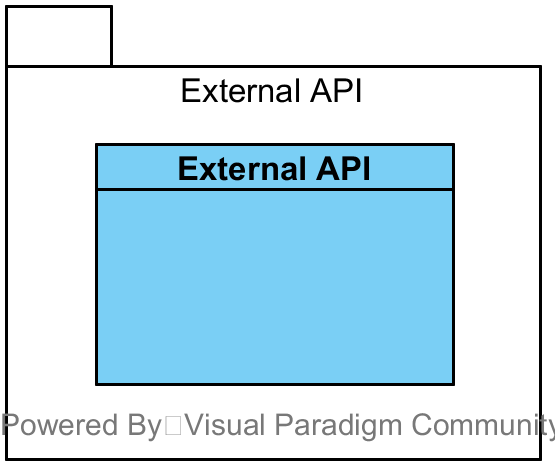
\includegraphics[height=5cm]{diagrammi_img/classi_e_package/api_esterne.png}
	\caption{Api\-::External\-Api}
\end{figure}
\end{samepage}
\textbf{Descrizione:}\\ 
Il package di chiamata delle API esterne aggiunge al framework la possibilità di effettuare internamente alla bubble chiamate di API REST di terze parti restituendo nella bubble memory il risultato di questa chiamata. \\
\textbf{Scopo:}\\
Si occupa di interfacciarsi con servizi terzi restituendo il risultato alla bubble memory.\\

\begin{samepage}
\paragraph{Api\-::Partecipants}\label{api-partecipanti}\mbox{}\\
\nopagebreak
\begin{figure}[H]
	\centering
	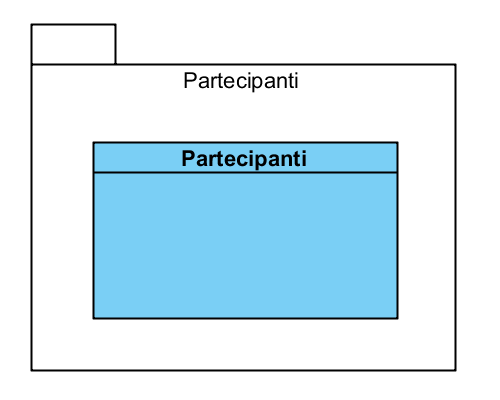
\includegraphics[height=5cm]{diagrammi_img/classi_e_package/api_partecipanti.png}
	\caption{Api\-::Partecipants}
\end{figure}
\end{samepage}
\textbf{Descrizione:}\\ 
Gestisce le operazioni di gestione degli utenti e delle loro interazioni.\\
\textbf{Scopo:}\\
Questo package garantisce alla bubble la possibilità di avere accesso alla lista dei partecipanti alla chat e uno storico delle interazioni di ciascuno con essa.

\begin{samepage}
\paragraph{Api\-::DbOperations}\label{api-db}\mbox{}\\
\nopagebreak
\begin{figure}[H]
	\centering
	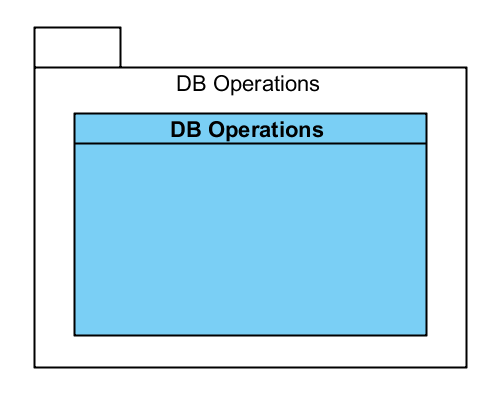
\includegraphics[height=5cm]{diagrammi_img/classi_e_package/api_operazionidb.png}
	\caption{Api\-::DbOperations}
\end{figure}
\end{samepage}
\textbf{Descrizione:}\\
Nel package di operazioni sul DB sono racchiuse le funzionalità per connettersi ad un database non relazionale ed effettuare al suo interno operazioni di lettura e di scrittura.\\
\textbf{Scopo:}\\
Oltre alle normali operazioni sul database l'utente avrà la possibilità di utilizzare un database esterno.

\begin{samepage}
\paragraph{Api\-::Input\-Limitation}\label{api-limiti}\mbox{}\\
\nopagebreak
\begin{figure}[H]
	\centering
	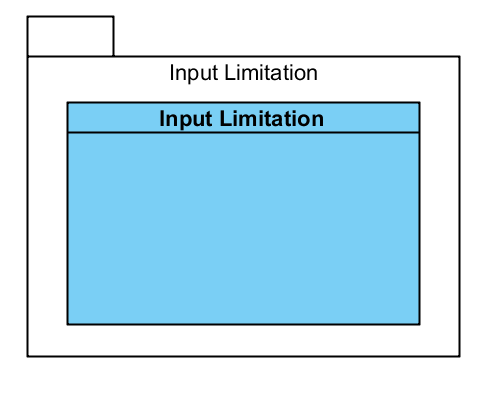
\includegraphics[height=5cm]{diagrammi_img/classi_e_package/api_limitinput.png}
	\caption{Api\-::Input\-Limitation}
\end{figure}
\end{samepage}
\textbf{Descrizione:}\\
Controlla i vari input accettati dalle bubble, limitandone contenuto o numero di accessi.\\
\textbf{Scopo:}\\
In questo package sono contenute le funzionalità del framework relative alle limitazioni sull'input fornito alla bubble. Saranno quindi presenti metodi per consentire un numero limitato di interazioni pro capite con la bubble o un numero totale di interazioni effettuabili dagli utenti di Rocket.Chat che la utilizzino.\\
Saranno inoltre presenti dei metodi per verificare il match di un eventuale input testuale con un'espressione regolare e limitazioni sulla sua lunghezza massima. Nel caso l'input da validare sia in formato JSON (per esempio un valore ritornato dalla chiamata di un API REST esterna) è possibile verificare che al loro interno siano presenti determinate chiavi indicate.

\begin{samepage}
\paragraph{Api\-::Timing}\label{api-timing}\mbox{}\\
\nopagebreak
\begin{figure}[H]
	\centering
	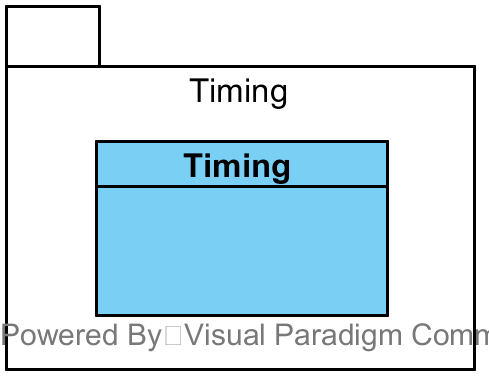
\includegraphics[height=5cm]{diagrammi_img/classi_e_package/api_timing.png}
	\caption{Api\-::Timing}
\end{figure}
\end{samepage}
\textbf{Descrizione:}\\
Il package di timing si occupa della pianificazione dell'esecuzione di determinati metodi ad orari prestabiliti all'interno della bubble.\\
\textbf{Scopo:}\\
Verrà utilizzato per la gestione di scadenze o eventi ripetuti in modo automatico.

\begin{samepage}
\paragraph{Api\-::File}\label{api-file}\mbox{}\\
\nopagebreak
\begin{figure}[H]
	\centering
	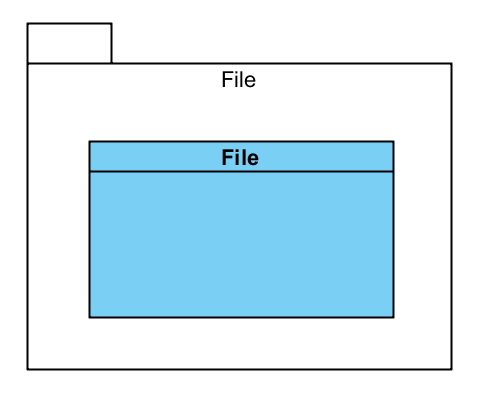
\includegraphics[height=5cm]{diagrammi_img/classi_e_package/api_file.png}
	\caption{Api\-::File}
\end{figure}
\end{samepage}
\textbf{Descrizione:}\\ 
Il package gestisce l'interazione della bubble con dei file.\\ 
\textbf{Scopo:}\\
Verrà usato come descritto nei casi d'uso per convertire del testo in PDF e salvare il file così prodotto.

\begin{samepage}
\paragraph{Api\-::Json\-Control}\label{api-json}\mbox{}\\
\nopagebreak
\begin{figure}[H]
	\centering
	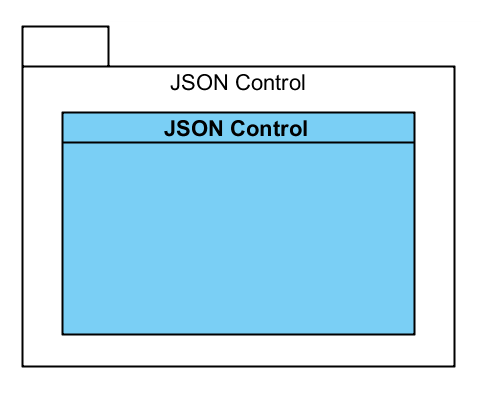
\includegraphics[height=5cm]{diagrammi_img/classi_e_package/api_json.png}
	\caption{Api\-::Json\-Control}
\end{figure}
\end{samepage}
\textbf{Descrizione:}\\ 
Il package permette il controllo di file JSON secondo uno schema specificato.\\ 
\textbf{Scopo:}\\
Verrà usato per verificare che il JSON prodotto sia conforme ad uno schema precedentemente fornito.

\begin{samepage}
\paragraph{Api\-::match\-Regular\-Expr}\label{api-regexpr}\mbox{}\\
\nopagebreak
\begin{figure}[H]
	\centering
	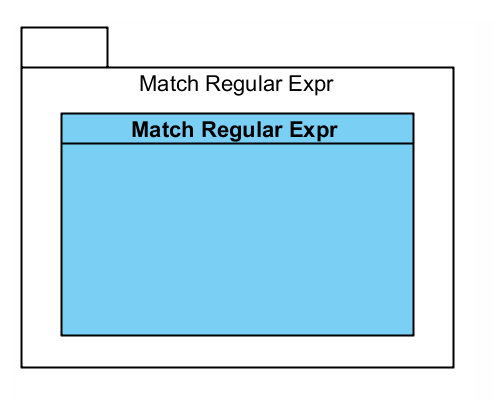
\includegraphics[height=5cm]{diagrammi_img/classi_e_package/api_matchex.png}
	\caption{Api\-::match\-Regular\-Expr}
\end{figure}
\end{samepage}
\textbf{Descrizione:}\\ 
Il package permette di effettuare confronti con espressioni regolari.\\ 
\textbf{Scopo:}\\
Verrà usato per controllare l'input inserito dall'utente.

\subsection{Controller}
La componente del Controller è costituita dalla classe Generic\-Bubble che si occupa di connettere le varie funzionalità offerte nella parte di Model con i rispettivi input ed output contenuti nella parte di View. Un utente del framework avrà la possibilità di definire e costruire la propria bolla all’interno di questo elemento. Potrà quindi inserire le interfacce offerte dalla GUI e connettere gli eventuali input di quest’ultime con delle componenti funzionali. Queste ultime potranno essere definite dall’utente stesso oppure scelte tra quelle disponibili. 
L’insieme di questi elementi e le loro interazioni definiranno il comportamento dell’istanza della Bubble creata dall’utente.
\begin{samepage}
\subsubsection{Controller\-::Generic\-Bubble}\label{fm-generica}
\nopagebreak
\begin{figure}[H]
	\centering
	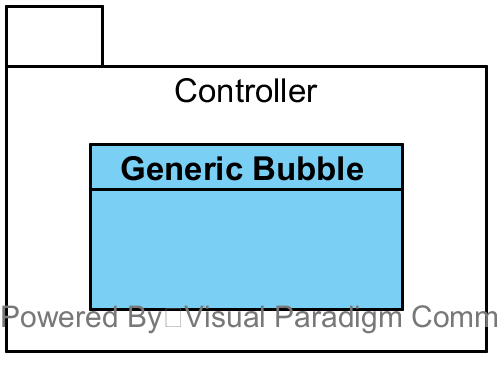
\includegraphics[height=5cm]{diagrammi_img/classi_e_package/bubble_generica.png}
	\caption{Controller\-::Generic\-Bubble}
\end{figure}
\end{samepage}
\textbf{Descrizione:}\\
La classe Generic Bubble permette di istanziare e gestire il flusso di dati tra la parte di interfaccia e la parte funzionale di una bubble.\\
\textbf{Scopo:}\\
Questa bolla gestisce le comunicazioni tra l’interfaccia e la parte di business logic. Invia gli input ricevuti alla rispettiva componente logica ed invia all’interfaccia gli eventuali output secondo le direttive fornite dall’utente.


\begin{samepage}
\subsection{View}
\nopagebreak
\begin{figure}[H]
	\centering
	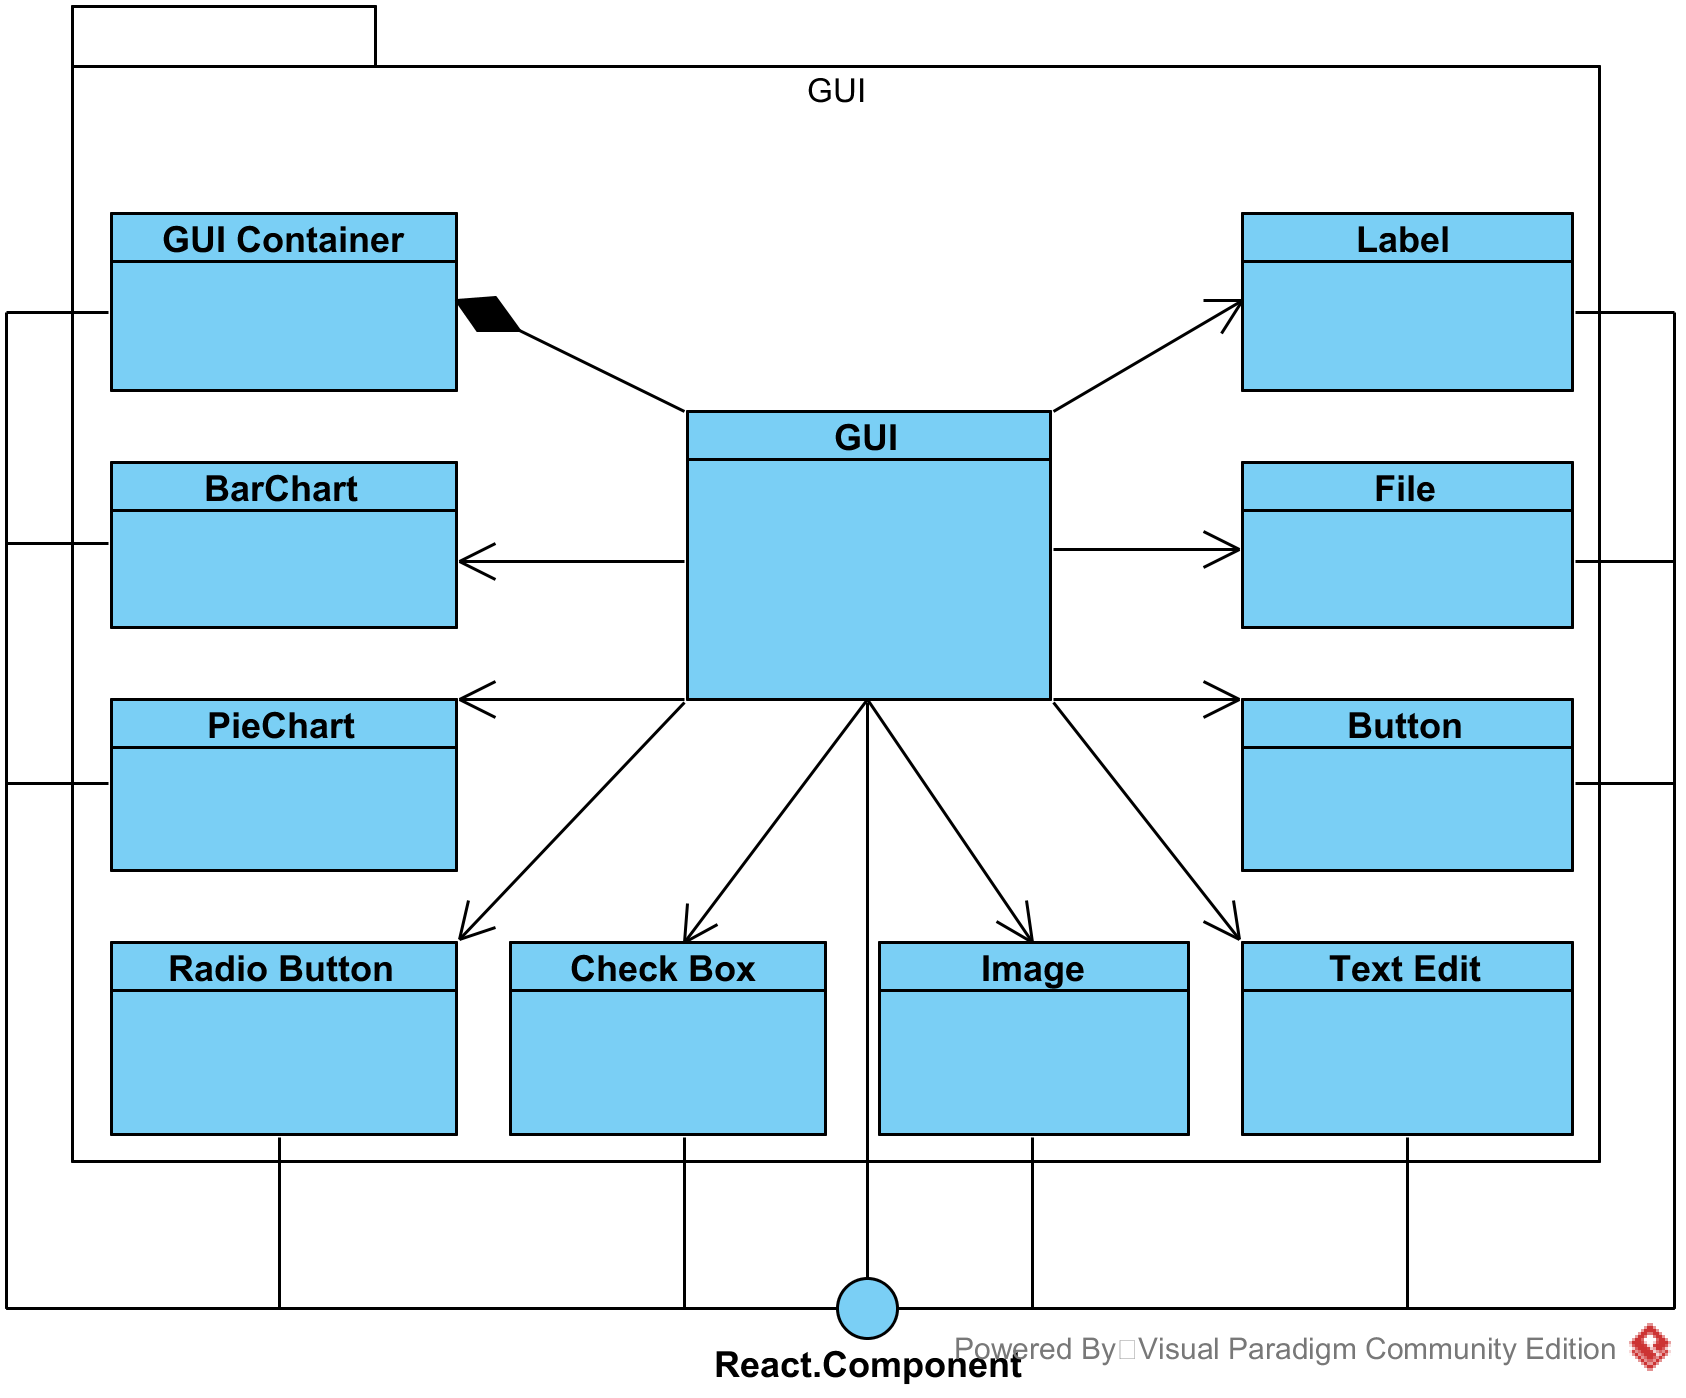
\includegraphics[width=14cm]{diagrammi_img/classi_e_package/gui_classes.png}
	\caption{View}
\end{figure}
\end{samepage}
\textbf{Descrizione:}\\
La parte di View dedicata alla gestione dell'interfaccia utente del framework è strutturata come mostrato nel diagramma delle classi riportato sopra.
Ogni elemento della GUI, come Button, TextEdit o Label, implementa l'interfaccia GUI, specificando opportunamente le funzioni a seconda che gli elementi siano di output o di input.\\
Gli elementi della GUI possono essere inseriti e raggruppati in un contenitore. In questo modo il Controller potrà organizzare in modo più semplice lo scambio di informazioni tra la parte Model e quella View, inserendo diversi elementi di GUI relativi ad una specifica funzionalità in un unico container.

\subsubsection{Classi}

\paragraph{View\-::Gui}\label{gui}\mbox{}\\
\textbf{Descrizione:}\\
L'interfaccia GUI racchiude i dati riguardanti la visibilità e l'aggiornamento. Offre le funzionalità di gestione dell'evento che andranno poi specificate in ogni classe che implementerà questa interfaccia.\\
\textbf{Utilizzo:}\\
Questa classe viene usata per gestire gli eventi degli elementi grafici.

\paragraph{View\-::Gui\-::Container}\label{gui-container}\mbox{}\\
\textbf{Descrizione:}\\
La classe contiene una collezione di uno o più elementi della GUI.\\ 
\textbf{Utilizzo:}\\
Questa classe permette l'inserimento, la manipolazione e la rimozione di elementi dall'interno della collezione della GUI. 

\paragraph{View\-::Gui\-::Label}\label{gui-label}\mbox{}\\
\textbf{Descrizione:}\\
La classe Label offre all'interno del framework la possibilità di utilizzare l'equivalente presente in HTML.\\
\textbf{Utilizzo:}\\
Questa classe offre la possibilità di renderizzare un output nella bubble.\\
\textbf{Relazioni con le altre classi:}\\
Questa classe rappresenta un elemento grafico, deriva da GUI e ne eredita i metodi.\\

\paragraph{View\-::Gui\-::File}\label{gui-file}\mbox{}\\
\textbf{Descrizione:}\\
Componente progettato per consentire alla bubble e al suo utilizzatore finale l'interazione con file generici.\\
\textbf{Utilizzo:}\\
Consente il caricamento di file nella bubble da parte dell'utente e permette alla stessa di rendere file generici disponibili ai suoi utilizzatori.\\
\textbf{Relazioni con le altre classi:}\\
Questa classe rappresenta un elemento grafico, deriva da GUI e ne eredita i metodi.\\

\paragraph{View\-::Gui\-::Button}\label{gui-button}\mbox{}\\
\textbf{Descrizione:}\\
Classe che permette di inserire nella bubble un oggetto di tipo Button, per permettere alla stessa di interagire con i suoi utilizzatori.\\
\textbf{Utilizzo:}\\
Fornisce alla bubble la possibilità di interagire con l'utente suo utilizzatore mediante un bottone.\\
\textbf{Relazioni con le altre classi:}\\
Questa classe rappresenta un elemento grafico, deriva da GUI e ne eredita i metodi.\\

\paragraph{View\-::Gui\-::Text\-Edit}\label{gui-tedit}\mbox{}\\
\textbf{Descrizione:}\\
Classe volta a fornire una funzionalità di interazione con l'utente mediante la modifica di testo.\\
\textbf{Utilizzo:}\\
Consentire all'utente l'inserimento nella bubble di testo ove fosse necessario.\\
\textbf{Relazioni con le altre classi:}\\
Questa classe rappresenta un elemento grafico, deriva da GUI e ne eredita i metodi.\\

\paragraph{View\-::Gui\-::Text\-View}\label{gui-tview}\mbox{}\\
\textbf{Descrizione:}\\
Classe volta alla realizzazione di un elemento in grado di mostrare all'utente del testo non modificabile.\\
\textbf{Utilizzo:}\\
Consentire all'utente la visualizzazione di testo nella bubble.\\
\textbf{Relazioni con le altre classi:}\\
Questa classe rappresenta un elemento grafico, deriva da GUI e ne eredita i metodi.\\

\paragraph{View\-::Gui\-::Image}\label{gui-image}\mbox{}\\
\textbf{Descrizione:}\\
La classe permette di estendere le funzionalità della bubble mediante l'interazione con immagini.\\
\textbf{Utilizzo:}\\
Consentire nella bubble la visualizzazione di immagini.\\
\textbf{Relazioni con le altre classi:}\\
Questa classe rappresenta un elemento grafico, deriva da GUI e ne eredita i metodi.\\

\paragraph{View\-::Gui\-::Check\-Button}\label{gui-check}\mbox{}\\
\textbf{Descrizione:}\\
La classe CheckButton porta all'interno del framework la possibilità di utilizzare l'equivalente presente in HTML.\\
\textbf{Utilizzo:}\\
L'utilizzo di questa classe è quello di fornire un bottone selezionabile.\\
\textbf{Relazioni con le altre classi:}\\
Questa classe rappresenta un elemento grafico, deriva da GUI e ne eredita i metodi.\\

\paragraph{View\-::Gui\-::Radio\-Button}\label{gui-radio}\mbox{}\\
\textbf{Descrizione:}\\
La classe RadioButton porta all'interno del framework la possibilità di utilizzare l'equivalente presente in HTML.\\
\textbf{Utilizzo:}\\
L'utilizzo di questa classe è quello di fornire un bottone selezionabile in modo esclusivo.\\
\textbf{Relazioni con le altre classi:}\\
Questa classe rappresenta un elemento grafico, deriva da GUI e ne eredita i metodi.\\

\paragraph{View\-::Gui\-::Pie\-Chart}\label{gui-pie}\mbox{}\\
\textbf{Descrizione:}\\
La classe PieChart porta all'interno del framework la possibilità di utilizzare grafici a torta.\\
\textbf{Utilizzo:}\\
L'utilizzo di questa classe è quello di fornire un grafico a torta per l'elaborazione grafica di dati.\\
\textbf{Relazioni con le altre classi:}\\
Questa classe rappresenta un elemento grafico, deriva da GUI e ne eredita i metodi.\\

\paragraph{View\-::Gui\-::Bar\-Chart}\label{gui-bar}\mbox{}\\
\textbf{Descrizione:}\\
La classe BarChart porta all'interno del framework la possibilità di utilizzare grafici a istogramma.\\
\textbf{Utilizzo:}\\
L'utilizzo di questa classe è quello di fornire un grafico a istogramma per l'elaborazione grafica di dati.\\
\textbf{Relazioni con le altre classi:}\\
Questa classe rappresenta un elemento grafico, deriva da GUI e ne eredita i metodi.\\